\chapter{Exploiting uncertainty of the Bellman operator components to deal with highly stochastic problems}\label{C:rq}
It is well known that a key issue of \gls{rl} applications is the accuracy of the estimation of the action-value with a limited number of samples. Although most algorithms guarantee the convergence of the estimates of the action values to the optimal values with infinite samples, in practice the presence of stochastic components leads to slow learning. Actually, most real-world problems have significant sources of stochasticity: the environment may have stochastic transitions and this may affect the estimation of the effectiveness of an action; most of the times it is necessary to use stochastic policies to guarantee that all states are potentially visited infinitely many times; the reward function is often corrupted by noisy observations and, in other cases, the reward function is stochastic itself. Moreover, it usually happens that some deterministic environments are partially observable and, thus, are perceived by the agent as stochastic decision processes (e.g. Blackjack).

Since Monte Carlo estimates of action values are affected by the high variance of returns, the most successful \gls{rl} algorithms are based on bootstrapping (e.g. $Q$-Learning \cite{watkins1989learning}), which trades off the variance of the estimation with a consistent, but biased estimator. However, with a finite number of samples, the bias of the estimates could be significantly relevant when propagating the action-values to the next state and, recursively, to all other states. Recent works tried to deal with this issue, in particular by focusing on the estimation of the \gls{mev}, as discussed in Chapter~\ref{C:mev}. 

However, an inaccurate estimation of the action value function does not always imply poor performance; indeed, most policies do not depend on the accuracy of the action-values, but, instead, rely on their ordering. Starting from these considerations, we address this problem from another point of view. Indeed, we do not focus on the estimation of the \gls{mev}, but we care about weighing the new samples according to the uncertainty of current estimates. 
We consider that it is not sufficient to accurately estimate the \gls{mev} of the $Q$-function of the next state, but we also need to analyze how this information is propagated to other states. The problem of dealing with the uncertainty and the propagation of information across the states of the \gls{mdp} has been addressed in many works on \gls{rl}~\cite{mohagheghi2007proportional, Tewari2007}. Some of them consist in tuning the meta-parameters of the learning process according to uncertainty, e.g. the dynamic changes of the environment~\cite{schweighofer2003meta, Kobayashi2009, yoshida2013reinforcement}.

The interesting aspect of this approach is that any \gls{mev} estimator can be used and can be easily extended to an on-policy scenario. Since we believe that the choice of the estimator is not a relevant issue in our approach, we choose the \gls{me} as it is the most common.

\section{Preliminaries}
Recalling the optimal action-value function
\begin{align}
 Q^*(s,a)=\underset{\strut\mathclap{s'\sim \mathcal{P}(\cdot|s,a)}}{\mathbb{E}}\left[ r(s,a,s')+\gamma\max_{a'} Q^*(s',a')\right],
 \label{eq:qopt}
\end{align}
as the expected value is a linear operator, we can always write (\ref{eq:qopt}) as:
\begin{align}
 Q^*(s,a)=\underset{\strut\mathclap{s'\sim \mathcal{P}(\cdot|s,a)}}{\mathbb{E}}\left[ r(s,a,s')\right]+\underset{\strut\mathclap{s'\sim \mathcal{P}(\cdot|s,a)}}{\gamma\mathbb{E}}\left[ \max_{a'} Q^*(s',a')\right].
 \label{eq:qdec}
\end{align}

Now, let us define two functions, $\tilde{R}$ and $\tilde{Q}$, as:
\begin{align}
 \tilde{R}(s,a)&=\underset{\strut\mathclap{s'\sim \mathcal{P}(\cdot|s,a)}}{\mathbb{E}}\left[ r(s,a,s')\right], \nonumber\ \\
 \tilde{Q}(s,a)&=\underset{\strut\mathclap{s'\sim \mathcal{P}(\cdot|s,a)}}{\mathbb{E}}\left[\max_{a'} Q^*(s',a')\right].
 \label{eq:rqtilde}
\end{align}
We can give an interpretation of these two functions: $\tilde{R}(s,a)$ is the expected immediate reward of action $a$ in state $s$; $\tilde{Q}(s,a)$ is the expected discounted return of the states reached after performing action $a$ in state $s$ (i.e. the expected gain of the reached state).
We can now write the optimal value function as:
\begin{align}
 Q^*(s,a)=\tilde{R}(s,a)+\gamma\tilde{Q}(s,a).
 \label{eq:qdecrqtilde}
\end{align}

Our approach shifts the focus of the \gls{rl} task from finding a good estimator for the optimal action-value function, to the task of finding good estimators for $\tilde{R}$ and $\tilde{Q}$. The main motivation is that the sources of uncertainty of the two components of the action-value function are different: $\tilde{R}$ only depends on the transition and reward models, while $\tilde{Q}$ depends also on the optimal policy.
\section{The proposed method}
In the following section, we derive our method from (\ref{eq:qdecrqtilde}). We propose the general schema, using the \gls{me}, and we show the relationships with the standard $Q$-Learning update. We call this method $RQ$-Learning as it decomposes the \gls{td}-Error into a reward component and an action-value component.

\subsection{Decomposition of the TD error}
The standard $Q$-Learning algorithm, given the tuple $(s,a,r,s')$, computes the temporal difference error w.r.t. the current action-value estimates, and then updates such estimate proportionally to the error. The amount of correction in the direction of the new sample is measured by the learning rate: if the learning rate is $1$, the new sample substitutes the old estimate; if the learning rate is $0$, the new sample is discarded and the old estimate is kept unchanged. 
As shown in (\ref{eq:qdecrqtilde}) the action-value function could be decomposed into two different components. Our method is based on the idea of giving separate estimates for these two components by computing the error w.r.t. each component of the action-value function, instead of computing the \gls{td} error:
\begin{align}
\tilde{R}_{t+1}(s,a) & \leftarrow\tilde{R}_t(s,a)+\alpha_t(R(s,a,s')-\tilde{R}_t(s,a)), \label{eq:rtilupdedate}\\
\tilde{Q}_{t+1}(s,a) & \leftarrow\tilde{Q}_t(s,a)+\beta_t(\max_{a'}Q_t(s',a')-\tilde{Q}_t(s,a)).
\label{eq:qtildeupdate}
\end{align}
Separating the two components of the value function can be useful, as the two components have inherently different sources of stochasticity. Moreover, the information stored in $\tilde{R}$ is local to each state-action pair and does not contain the uncertainty of estimating other states. Instead, the information stored in $\tilde{Q}$ depends only on the action-value function of the states that could be reached after performing action $a$ in state $s$, which depends, recursively, on the other action-value functions. It is clear that the propagation of uncertain values affects only the $\tilde{Q}$ component.
As the actual action-value function is the sum of the two estimates, we can write an equivalent update for the Q-value:
\begin{align}
Q_{t+1}(s,a)\leftarrow&\tilde{R}_t(s,a)+\alpha_t(R(s,a,s')-\tilde{R}_t(s,a)) \nonumber\\
  & +\gamma\left(\tilde{Q}_t(s,a)+\beta_t(\max_{a'}Q_t(s',a')-\tilde{Q}_t(s,a))\right) \nonumber\\
= & Q_t(s,a)+\alpha_t(R(s,a,s')-\tilde{R}_t(s,a)) \nonumber\\
  & +\gamma\beta_t(\max_{a'}Q_t(s',a')-\tilde{Q}_t(s,a)).
 \label{eq:cumulativeupdate}
\end{align}

\subsection{Analysis of the decomposed update}
Now, we discuss the relationship of our method with the standard temporal difference methods. Let $t$ be the learning step. As a first step of our analysis we can consider the simplest case $\alpha_t=\beta_t$, $\forall t$ by combining (\ref{eq:cumulativeupdate}) and (\ref{eq:qdecrqtilde}) we obtain:
\begin{align}
Q_{t+1}(s,a) \leftarrow & Q_t(s,a)+\alpha_t(R(s,a,s')+\gamma\max_{a'}Q_t(s',a') - Q_t(s,a)).
\end{align}
That is the classical $Q$-Learning update. 

We consider now the setting $\alpha_t\geq\beta_t>0$, $\forall t$. Let $\beta_t=\delta_t\alpha_t$, we obtain:
\begin{align}
Q_{t+1}(s,a) \leftarrow & Q_t(s,a)+\alpha_t(R(s,a,s')+\gamma\delta_t \max_{a'}Q_t(s',a') \nonumber\\
  & -(\tilde{R}_t(s,a)+\gamma\delta_t\tilde{Q}_t(s,a))) \nonumber\\
= & Q_t(s,a)+\alpha_t(R(s,a,s')+\gamma_t'\max_{a'}Q_t(s',a') \nonumber\\
  & -(\tilde{R}_t(x,u)+\gamma_t'\tilde{Q}_t(s,a))) \nonumber\\
= & Q_t(s,a)+\alpha_t((R(s,a,s')+\gamma_t'\max_{a'}Q_t(s',a')) \nonumber\\
  & - Q_t'(s,a))
\end{align}
with $\gamma_t'=\gamma\delta_t$. Notice that $Q_t'(s,a)$ is the Q-value at time step $t$, but computed with a different discount factor. If $\beta_t=\delta_t\alpha_t$, then we can see our method as a variable discount factor learning. If we consider that $\delta_t$ increases monotonically in the interval $[0,1]$, our method works by increasing the effective horizon at each step starting from trying to solve a greedy myopic problem and moving towards the real one.
Similar approaches have been used in practice to solve infinite-horizon problems when the discount factor $\gamma \approx 1$ ~\cite{crites1996improving, bao2008infinite, franccois2015discount}.

Finally, we can observe that, if the reward function and the transition model are deterministic, we can set $\alpha=1$ and consider only $\beta_t=\delta_t$.

\subsection{Variance dependent learning rate}
To improve the quality of the estimation, we would like to weigh the error of each sample w.r.t. the current estimate depending on how much we trust the current value of our estimate. Thus, we propose a learning rate that depends on the variance of the current variable estimate.

First of all, we need to compute the variance of each estimator. To perform such computation, we must assume that the learning rate is independent of the data. This assumption is needed to have a closed form for the variance of the estimator, and it works well in practice. We will also assume that the samples $X_i$ are i.i.d., with mean $\mu$ and variance $\sigma^2$. Consider the general form of the estimator:
\begin{align}
 \widetilde{X}_{n+1} = (1-\alpha_t)\widetilde{X}_{n}+\alpha_tX_{n}.
\end{align}
We now compute the expected value and the variance of this estimator:
\begin{align}
 \mathbb{E}\left[\widetilde{X}_{n+1}\right]& = \mu\sum_i^n \alpha_i \prod_{j=i+1}^{n} \left(1-\alpha_j\right)\\
 \mathrm{Var}\left[\widetilde{X}_{n+1}\right]& = \sigma^2\sum_i^n \alpha_i^2 \prod_{j=i+1}^{n} \left(1-\alpha_j\right)^2 = \sigma^2\omega
\end{align}
with $\omega=\sum_i^n \alpha_i^2 \prod_{j=i+1}^{n} \left(1-\alpha_j\right)^2$. Notice also that we can use the sample covariance $S_{n-1}$ of the random variable $X$ to estimate the real covariance $\sigma^2$. It is possible to compute incrementally way both the sample covariance, in the traditional way, and $\omega$:
\begin{align}
 \omega_{n+1}=(1-\alpha_n)^2\omega_n+\alpha_n^2.
\end{align}
A weak assumption of this model is that the variables are identically distributed. While this may be true for the reward function, if the \gls{mdp} is stationary, this is not true for the action-value function values whose distribution is affected by the policy and by the current estimates of the other states. However, a good approximation could be to consider data collected in a time window in which the distribution is approximately stationary. Using this approach, we can compute the variance of the process in a given time window by forgetting the old values that can lead to a biased estimation of the current window variance. Although this approach is not formally correct, as the derivation of the variance estimates makes the assumption of i.i.d. variables, this approximation leads to very good results in practice as we show in the empirical Section \ref{S:empirical}.

Finally, we can choose a learning rate that depends on the covariance. Let $\sigma_e^2(t)$ be an estimate of $\mathrm{Var}\left[\widetilde{X}_{t}\right]$. We propose the following learning rate for each component of the action-value function:
\begin{align}\label{eq:alpha_eq}
 \alpha_t=\dfrac{\sigma_e^2(t)}{\sigma_e^2(t)+\eta}
\end{align}
where $\eta$ is the amount of the estimator variance for which the learning rate is $0.5$ (i.e. when $\sigma_e=\eta$ the learning rate is $0.5$). It can be seen as a soft threshold to tune the rate of decrease in the learning rate w.r.t. the estimator variance.

If we consider the case $\beta_t=\alpha_t\delta_t$, then we have to use a different learning rate. As we want an increase in the discount factor faster than the decrease in the general learning rate, we can use an exponentially increasing learning rate for the delta parameter:
\begin{align}\label{eq:delta_eq}
 \delta_t = e^{\frac{\sigma_e^2}{\eta}\log\frac{1}{2}},
\end{align}
where $\eta$ has the same interpretation as in~(\ref{eq:alpha_eq}) thanks to the $\log\frac{1}{2}$ factor.

\subsection{Discussion on convergence}
Convergence of the $Q$-Learning algorithm is guaranteed under some conditions, including some properties on the learning rates ~\cite{EvenDar2001, watkins1989learning}:
\begin{align}
 0 \leq \alpha_t < 1, \forall t\nonumber \\
 \lim_{N\rightarrow\infty} \sum_{t=1}^{N}\alpha_t & = \infty,\nonumber \\
 \lim_{N\rightarrow\infty} \sum_{t=1}^{N}\alpha_t^2 & < \infty. \label{eq:lr_cond}
\end{align}
To provide some preliminary results about the convergence of $RQ$-Learning and to motivate the choice of the formulas of learning rates $\alpha$ and $\delta$, we show that, under some assumptions, the proposed formulas (\ref{eq:alpha_eq}) (\ref{eq:delta_eq}) satisfy (\ref{eq:lr_cond}). Suppose that the variance of the estimator $\sigma_e^2(t)$ is the variance of the sample mean. It is well known, by the central limit theorem, that the variance of the sample mean is $\sigma_{\mu}(t)=\frac{\sigma^2}{t}$, where $\sigma$ is the variance of the process that generates the samples.
This assumption does not hold in general, as we can see from the formula of the learning rate; however, this is true for the sample mean, which is a special case of the generic estimator.

Now, just consider the learning rate proposed in (\ref{eq:alpha_eq}), replacing the variance of the sample mean into the variance of the estimator:
\begin{align}\label{eq:alpha_smv}
 \alpha_t=\frac{\sigma^2}{\sigma^2+\eta t}
\end{align}
it can be easily shown that:
\begin{align}
 \lim_{N\rightarrow\infty} \sum_{t=1}^{N}\frac{\sigma^2}{\sigma^2+\eta t} & = \infty, \\
 \lim_{N\rightarrow\infty} \sum_{t=1}^{N}\left(\frac{\sigma^2}{\sigma^2+\eta t}\right)^2 & < \infty.
\end{align}
Now, consider $\beta_t=\alpha_t\delta_t$. In this scenario, we propose an exponential learning rate. Let be $\alpha_t=\frac{1}{t}$ for simplicity, and consider the learning rate (\ref{eq:delta_eq}) to replace the sample mean into the variance of the estimator:
\begin{align}\label{eq:beta_delta_smv}
 \beta(t) = \frac{1}{t}e^{\frac{\sigma^2}{\eta t}\log\frac{1}{2}}.
\end{align}
Then:
\begin{align}
 \lim_{N\rightarrow\infty} \sum_{t=1}^{N}\frac{1}{t}e^{\frac{\sigma^2}{\eta t}\log\frac{1}{2}} & = \infty, \\
 \lim_{N\rightarrow\infty} \sum_{t=1}^{N}\left(\frac{1}{t}e^{\frac{\sigma^2}{\eta t}\log\frac{1}{2}}\right)^2 & < \infty.
\end{align}
This analysis considers only the estimate of the variance of the sample mean. The analysis of the generic variance estimator is more complex, but we conjecture that convergence could be guaranteed under some mild conditions on $\eta$ and $\sigma$.

\begin{figure}[t]
\begin{minipage}{\columnwidth}
\centering
  \subfigure[$\alpha = \dfrac{1}{n(s,a)}$\label{F:hasselt_all_1}]{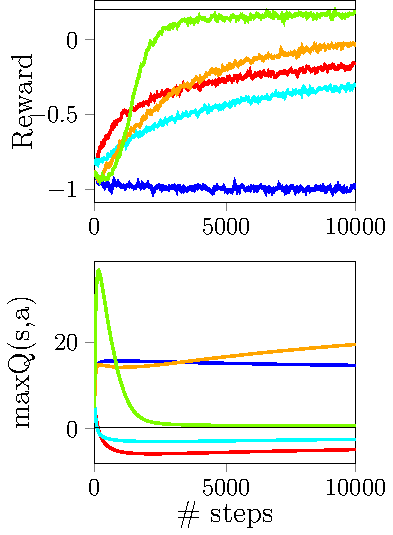
\includegraphics[scale=.7]{./img/allAlgs1.pdf}}
  \subfigure[$\alpha = \dfrac{1}{n(s,a)^{0.8}}$\label{F:hasselt_all_08}]{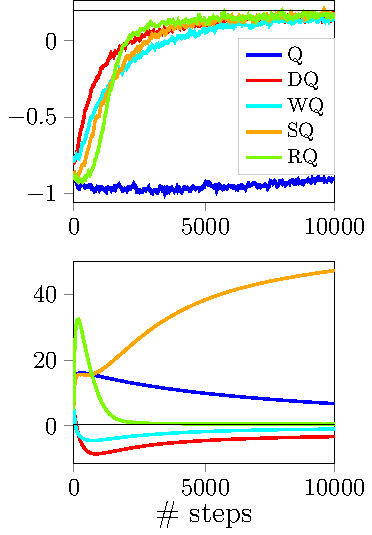
\includegraphics[scale=.7]{./img/allAlgs08.pdf}}
\end{minipage}
  \caption[Noisy Grid World algorithms comparison]{Mean reward per step (top) and maximum action-value estimate in the initial state (bottom) in the Noisy Grid World problem of all the other algorithms and of the best setting of $RQ$-Learning for this experiment. Results are averaged over $10000$ experiments.}
  \label{F:hasselt_all}
\end{figure}
\begin{figure}[t]
\begin{minipage}{\columnwidth}
\centering
  \subfigure[$\alpha = \dfrac{1}{n(s,a)}$\label{F:hasselt_qdec_1}]{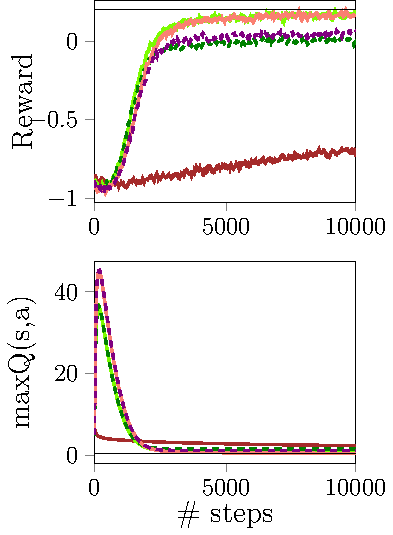
\includegraphics[scale=.7]{./img/QDecs1.pdf}}
  \subfigure[$\alpha = \dfrac{1}{n(s,a)^{0.8}}$\label{F:hasselt_qdec_08}]{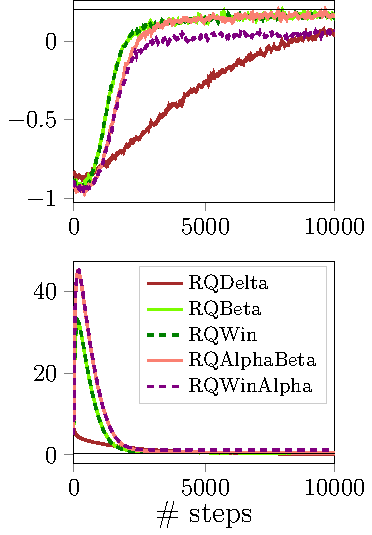
\includegraphics[scale=.7]{./img/QDecs08.pdf}}
\end{minipage}
  \caption[Noisy Grid World $RQ$-Learning variants comparison - 1]{Mean reward per step (top) and maximum action-value estimate in the initial state (bottom) in the Noisy Grid World problem of the best setting of $RQ$-Learning for this experiment together with other less effective setting of $RQ$-Learning. Results are averaged over $10000$ experiments.}
  \label{F:hasselt_QDecs}
\end{figure}
\begin{figure}[t]
\begin{minipage}{\columnwidth}
\centering
  \subfigure[$RQ$-Learning\label{F:hasselt_qdectol}]{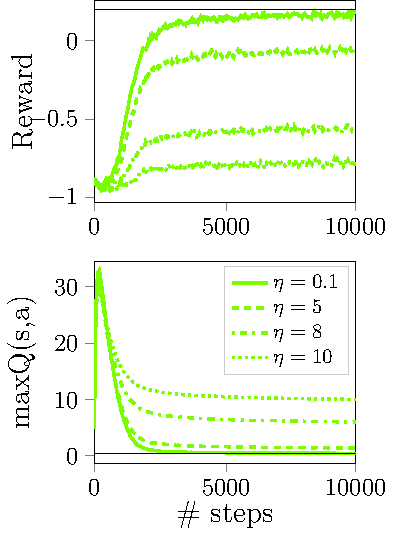
\includegraphics[scale=.7]{./img/QDecHasselt.pdf}}
  \subfigure[Windowed $RQ$-Learning\label{F:hasselt_qdecwintol}]{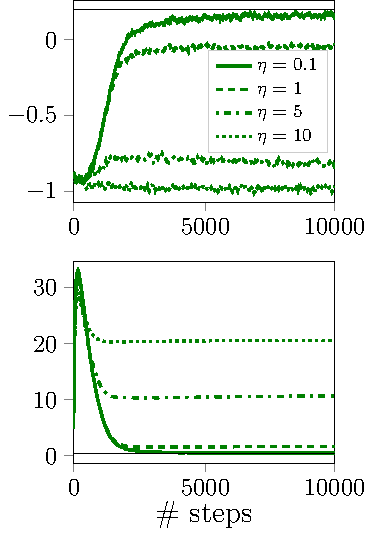
\includegraphics[scale=.7]{./img/QDecWinHasselt.pdf}}
\end{minipage}
  \caption[Noisy Grid World $RQ$-Learning variants comparison - 2]{Mean reward per step (top) and maximum action-value estimate in the initial state (bottom) in the Noisy Grid World problem of $RQ$-Learning (Figure \ref{F:hasselt_qdectol}) and windowed $RQ$-Learning (Figure \ref{F:hasselt_qdecwintol}) with different values of $\eta$ and $k = 0.8$. Results are averaged over $10000$ experiments.}
  \label{F:hasselt_QDecTol}
\end{figure}

\section{Experimental results}\label{S:empirical}
We compare $RQ$-Learning against $Q$-Learning \cite{watkins1989learning}, Double $Q$-Learning \cite{van2010double}, Weighted $Q$-Learning \cite{deramo2016estimating} and Speedy $Q$-Learning\footnote{In these experiments we consider the asynchronous version of Speedy $Q$-Learning.} \cite{NIPS2011_4251} in three discrete \glspl{mdp}. We choose this set of algorithms because we want to analyze the impact of the maximum expected value estimator in the learning process. Indeed, while \cite{van2010double} strongly suggests that a negatively biased estimator should be used to deal with stochastic \glspl{mdp}, the  empirical results, reported in the following, show that positively biased estimators are able to achieve better performance in highly stochastic problems as well. Instead, we show that the main point is to exploit the data in the best way, in particular in the estimation of the action-value, giving higher relevance to more recent samples. We conjecture that the trade-off between keeping the old estimate and updating it with the new one is the key issue in highly stochastic environments. Both $RQ$-Learning and Speedy $Q$-Learning exploit this idea; in particular, the latter uses an increasing learning rate on the difference between the target computed with the current estimation and the one computed with the previous estimation, while $RQ$-Learning weigh the update considering the uncertainty of the current estimation.

We analyze the performance of $RQ$-Learning with different choices of learning rates. All the other algorithms use a decaying learning rate $\alpha(s, a) = \frac{1}{n(s, a)^{k}}$ where $n(s, a)$ and $k$ are respectively the number of updates for each action $a$ in state $s$ and a coefficient to tune the rate of decay.\footnote{Assuming that Double $Q$-Learning splits the action-value table in a table A and a table B, also the learning rate is split in $\alpha_A(s, a) = \frac{1}{n_A(s, a)^{k}}$ and $\alpha_B(s, a) = \frac{1}{n_B(s, a)^{k}}$, where $n_A(s, a)$ and $n_B(s, a)$ are the number of updates for each action $a$ in state $s$, respectively in table A and table B.}

\subsection{Noisy Grid World}
This environment, proposed in \cite{van2010double}  and \cite{deramo2016estimating}, consists of a $3 \times 3$ grid with the initial position in the lower-left cell and the goal state in the upper-right cell. Every action performed in a non-goal state obtains a reward $-12$ and $10$ with equal probability. In the goal state, each action obtains a reward of $5$ and terminates the episode. The discount factor is $\gamma = 0.95$. The policy is $\varepsilon$-greedy with $\varepsilon = \frac{1}{\sqrt{n(s)}}$, where $n(s)$ is the number of  visits of the state $s$. The optimal average reward per step is $0.2$ and the maximum action-value function of the initial state is $5\gamma^4 - \sum_{k=0}^3 \gamma^k \approx 0.36$.

Figure \ref{F:hasselt_all} shows the average reward per step and the approximation of the maximum action-value in the initial state computed by the other algorithms and $RQ$-Learning with $\alpha$ as used by the other algorithms, but with the separated variance-dependent learning rate $\beta$ for the action-value estimate using $\eta = 1$. Notice how the performance of $RQ$-Learning for the reward is the best one (except for $k=0.8$ where all the algorithms perform similarly) and, also, how the estimate of the action-value is the best one. With $k=1$, Speedy $Q$-Learning outperforms both Double $Q$-Learning and Weighted $Q$-Learning considering the average reward per step, even with a divergent estimate of the action-value function. This is an empirical evidence of our conjecture: the bias of the estimation is not necessarily correlated to performance. Moreover, as expected, the performance of $RQ$-Learning is not affected by the exponent used in the learning rate. The other algorithms achieve optimal performance only in the setting with the highest learning rate, confirming the advantage of giving more importance to the newer samples.

In Figure \ref{F:hasselt_QDecs}, we compare different variants of $RQ$-Learning: ``RQBeta'' is the same configuration used in Figure \ref{F:hasselt_all}; ``RQDelta'' uses $\beta = \alpha \delta$ with $\eta = 1$; ``RQWin'' uses a windowed estimation of the variance with a window of length $50$ and $\eta = 0.5$. ``RQAlphaBeta'' uses a variance-dependent learning rate also for $\alpha$ with $\eta = 100$ and $\beta$ with $\eta = 1$; ``RQWinAlpha'' is the same as configuration of the previous one, but uses a windowed $\beta$ with $\eta = 0.5$. Note that $\eta$ has a larger value in configurations without windowed variance estimation because such configurations are likely to overestimate the current variance of the process. The ``RQDelta'' configurations result in a cautious learning that leads to very slow improvements, but avoids the overestimation of the action-value slowly converging to the optimal value. While ``RQDelta'' performance is not comparable to other configurations of $RQ$-Learning, it still outperforms $Q$-Learning. The other configurations perform similarly to the best one.

In Figure \ref{F:hasselt_QDecTol} we show the same information as Figure \ref{F:hasselt_all} and \ref{F:hasselt_QDecs} for $RQ$-Learning with different values of $\eta$ to give a sense of how this parameter influences the learning process. It is clear how lower values of $\eta$ (i.e. a higher learning rate) let the results converge faster, confirming that a high value of the learning rate helps to speed up the learning process in highly stochastic environments like this.

\begin{figure}[t]
\begin{center}
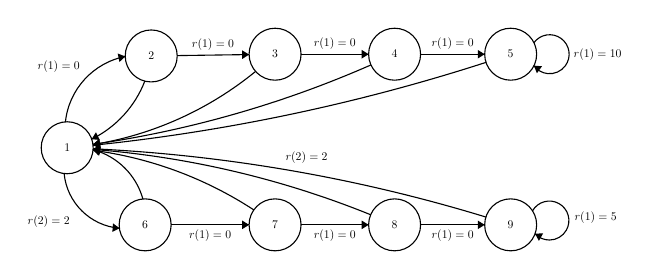
\begin{tikzpicture}[scale=0.11]
\tikzstyle{every node}+=[inner sep=0pt, style={scale=0.65}]
\draw [black] (10.4,-17.1) circle (3);
\draw (10.4,-17.1) node {$1$};
\draw [black] (20.1,-6.5) circle (3);
\draw (20.1,-6.5) node {$2$};
\draw [black] (34.4,-6.3) circle (3);
\draw (34.4,-6.3) node {$3$};
\draw [black] (48.2,-6.3) circle (3);
\draw (48.2,-6.3) node {$4$};
\draw [black] (61.6,-6.3) circle (3);
\draw (61.6,-6.3) node {$5$};
\draw [black] (19.4,-26) circle (3);
\draw (19.4,-26) node {$6$};
\draw [black] (34.4,-26) circle (3);
\draw (34.4,-26) node {$7$};
\draw [black] (48.2,-26) circle (3);
\draw (48.2,-26) node {$8$};
\draw [black] (61.6,-26) circle (3);
\draw (61.6,-26) node {$9$};
\draw [black] (10.195,-14.122) arc (-186.01298:-258.90993:8.628);
\fill [black] (17.12,-6.56) -- (16.23,-6.22) -- (16.43,-7.2);
\draw (11.87,-7.74) node [left] {$r(1)=0$};
\draw [black] (16.449,-26.391) arc (-94.70547:-174.65436:7.013);
\fill [black] (16.45,-26.39) -- (15.69,-25.83) -- (15.61,-26.82);
\draw (8.26,-24.87) node [below] {$r(2)=2$};
\draw [black] (13.375,-17.324) arc (75.15536:15.48481:8.153);
\fill [black] (13.37,-17.32) -- (14.02,-18.01) -- (14.28,-17.05);
\draw [black] (19.363,-9.401) arc (-21.12574:-63.79717:12.497);
\fill [black] (13.22,-16.11) -- (14.16,-16.2) -- (13.72,-15.31);
\draw [black] (32.152,-8.285) arc (-50.72552:-80.81899:39.653);
\fill [black] (13.38,-16.73) -- (14.25,-17.1) -- (14.09,-16.11);
\draw [black] (45.468,-7.539) arc (-66.30261:-81.8066:123.727);
\fill [black] (13.37,-16.71) -- (14.24,-17.09) -- (14.09,-16.1);
\draw [black] (58.752,-7.242) arc (-72.09117:-84.0864:221.864);
\fill [black] (13.39,-16.81) -- (14.23,-17.23) -- (14.13,-16.23);
\draw [black] (13.385,-17.393) arc (82.46666:56.84042:44.631);
\fill [black] (13.39,-17.39) -- (14.11,-17.99) -- (14.24,-17);
\draw [black] (13.394,-17.292) arc (85.54014:67.96192:107.716);
\fill [black] (13.39,-17.29) -- (14.15,-17.85) -- (14.23,-16.86);
\draw [black] (13.398,-17.219) arc (87.26949:73.00835:185.371);
\fill [black] (13.4,-17.22) -- (14.17,-17.76) -- (14.22,-16.76);
\draw (38.03,-18.9) node [above] {$r(2)=2$};
\draw [black] (22.4,-26) -- (31.4,-26);
\fill [black] (31.4,-26) -- (30.6,-25.5) -- (30.6,-26.5);
\draw (26.9,-26.5) node [below] {$r(1)=0$};
\draw [black] (37.4,-26) -- (45.2,-26);
\fill [black] (45.2,-26) -- (44.4,-25.5) -- (44.4,-26.5);
\draw (41.3,-26.5) node [below] {$r(1)=0$};
\draw [black] (51.2,-26) -- (58.6,-26);
\fill [black] (58.6,-26) -- (57.8,-25.5) -- (57.8,-26.5);
\draw (54.9,-26.5) node [below] {$r(1)=0$};
\draw [black] (51.2,-6.3) -- (58.6,-6.3);
\fill [black] (58.6,-6.3) -- (57.8,-5.8) -- (57.8,-6.8);
\draw (54.9,-5.8) node [above] {$r(1)=0$};
\draw [black] (37.4,-6.3) -- (45.2,-6.3);
\fill [black] (45.2,-6.3) -- (44.4,-5.8) -- (44.4,-6.8);
\draw (41.3,-5.8) node [above] {$r(1)=0$};
\draw [black] (23.1,-6.46) -- (31.4,-6.34);
\fill [black] (31.4,-6.34) -- (30.59,-5.85) -- (30.61,-6.85);
\draw (27.23,-5.85) node [above] {$r(1)=0$};
\draw [black] (64.28,-4.977) arc (144:-144:2.25);
\draw (68.85,-6.3) node [right] {$r(1)=10$};
\fill [black] (64.28,-7.62) -- (64.63,-8.5) -- (65.22,-7.69);
\draw [black] (64.117,-24.39) arc (150.34019:-137.65981:2.25);
\draw (68.96,-25.15) node [right] {$r(1)=5$};
\fill [black] (64.41,-27.02) -- (64.86,-27.85) -- (65.35,-26.98);
\end{tikzpicture}
\end{center}
\caption{Structure of the Double Chain problem.}
\label{F:double-chain}
\end{figure}

\subsection{Double Chain}
\begin{figure*}[t]
\begin{minipage}{\textwidth}
\centering
  \subfigure[$\alpha = \dfrac{1}{n(s,a)}$\label{F:double_chain_1_1}]{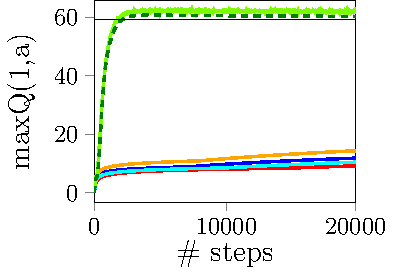
\includegraphics[scale=.55]{./img/v1-1.pdf}}
  \subfigure[$\alpha = \dfrac{1}{n(s,a)^{0.51}}$\label{F:double_chain_1_51}]{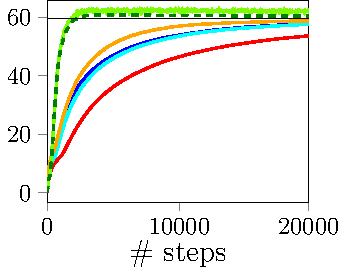
\includegraphics[scale=.55]{./img/v1-51.pdf}}
  \subfigure[$\alpha = \dfrac{1}{n(s,a)}$\label{F:double_chain_5_1}]{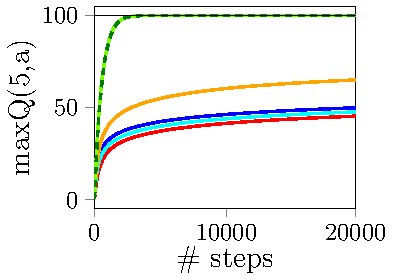
\includegraphics[scale=.55]{./img/v5-1.pdf}}
  \subfigure[$\alpha = \dfrac{1}{n(s,a)^{0.51}}$\label{F:double_chain_5_51}]{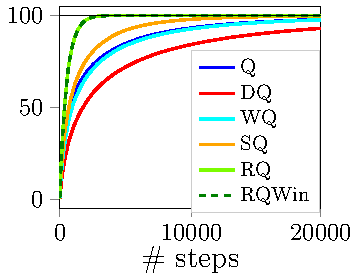
\includegraphics[scale=.55]{./img/v5-51.pdf}}
\end{minipage}
\caption[Double Chain results]{Maximum action-value estimate in the Double Chain problem in state $1$ (\ref{F:double_chain_1_1}, \ref{F:double_chain_1_51}) and state $5$ (\ref{F:double_chain_5_1}, \ref{F:double_chain_5_51}). Results are averaged over $500$ experiments.}
  \label{F:double_chain_q}
\end{figure*}
\begin{figure*}[t]
\begin{minipage}{\textwidth}
\centering
  \subfigure[$\alpha = \dfrac{1}{n(s,a)}$\label{F:lrs_1_1}]{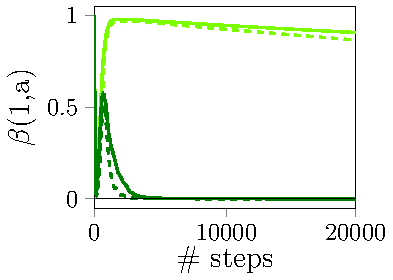
\includegraphics[scale=.55]{./img/lrs1-1.pdf}}
  \subfigure[$\alpha = \dfrac{1}{n(s,a)^{0.51}}$\label{F:lrs_1_51}]{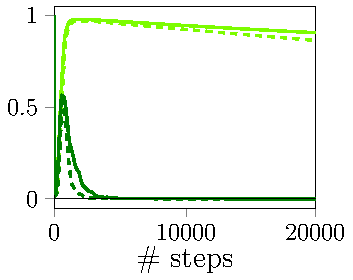
\includegraphics[scale=.55]{./img/lrs1-51.pdf}}
  \subfigure[$\alpha = \dfrac{1}{n(s,a)}$\label{F:lrs_5_1}]{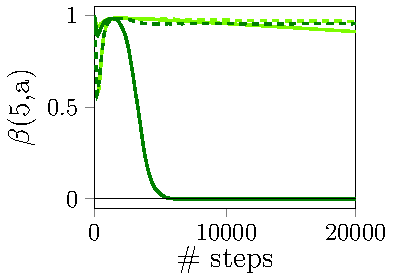
\includegraphics[scale=.55]{./img/lrs5-1.pdf}}
  \subfigure[$\alpha = \dfrac{1}{n(s,a)^{0.51}}$\label{F:lrs_5_51}]{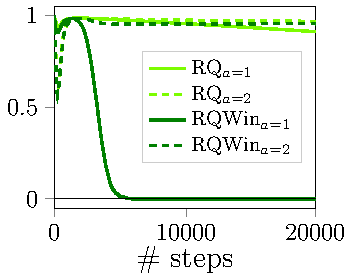
\includegraphics[scale=.55]{./img/lrs5-51.pdf}}
\end{minipage}
\caption[Learning rate adaptation in Double Chain problem]{Learning rate of the two actions in the Double Chain problem in state $1$ (\ref{F:lrs_1_1}, \ref{F:lrs_1_51}) and state $5$ (\ref{F:lrs_5_1}, \ref{F:lrs_5_51}) for $RQ$-Learning with and without windowed variance estimation. Results are averaged over $500$ experiments.}
  \label{F:double_chain_lr}
\end{figure*}
\begin{figure*}[t]
\begin{minipage}{\textwidth}
\centering
  \subfigure[$\alpha = \dfrac{1}{n(s,a)}$\label{F:max_a_1}]{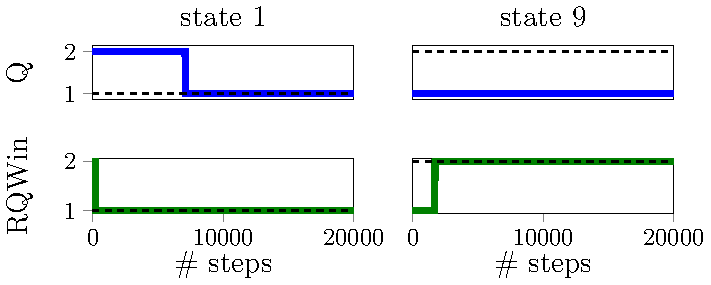
\includegraphics[scale=.55]{./img/max_a-1.pdf}}
  \subfigure[$\alpha = \dfrac{1}{n(s,a)^{0.51}}$\label{F:max_a_51}]{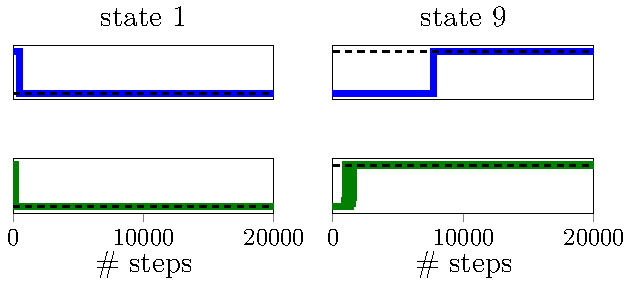
\includegraphics[scale=.55]{./img/max_a-51.pdf}}
\end{minipage}
\caption[Policy in Double Chain problem]{Action with maximum value in the Double Chain problem in state $1$ and state $9$ for $Q$-Learning and windowed $RQ$-Learning.}
  \label{F:max_a}
\end{figure*}
This is a problem proposed in \cite{Peters2010RelativeEP}, which consists of a Markov chain with two branches (Figure \ref{F:double-chain}). In state $1$, action $1$ yields a reward of $0$ and moves the agent into state $2$; action $2$ yields a reward of $2$ and moves the agent into state $6$. In all other states, action $2$ moves the agent into state $1$ and returns a reward of $2$; action $1$ moves the agent into the next state of the chain by returning a reward of $0$. In states $5$ and $9$, action $1$ yields a reward of $10$ and $5$ respectively. In all states, each action has a probability of success of $0.8$ and, if the action fails, the agent remains in the current state and yields a reward of $0$. The discount factor is $\gamma = 0.9$. The optimal policy is to take action $1$ in state from $1$ to $5$ and action $2$ in the other states. $RQ$-Learning uses $\eta = 10$. In this experiment we focus on the estimation of the action-value function, therefore we use a fully random policy to explore the environment.

Figure \ref{F:double_chain_q} shows the estimate of the maximum action value in state $1$ and $5$. State $5$ is the state with the highest maximum action-value. $RQ$-Learning approaches the optimal value faster than the other algorithms in both configurations. However, in state $1$, only $RQ$-Learning with windowed variance estimation converges to the optimal value because the non-windowed approach suffers from variance overestimation due to the fact that the distribution of the next action-values changes during learning; this issue, together with the stochasticity of the transitions, causes the oscillation of the estimate and a slow convergence rate. This behavior is highlighted in Figure \ref{F:double_chain_lr} where we show the learning rates of the action values in the considered states. While initially the learning rates are similar, the windowed learning rate converges to $0$, instead, in the non-windowed case, the learning rates decrease slowly. Note that in state $5$ the learning rate of action $2$ is almost stationary because of the complexity of the double chain structure. In this case, increasing $\eta$ can speedup the decreasing in the learning rate.

In this experiment, $RQ$-Learning not only approximates the value function very well, but is also able to converge to the optimal policy faster than the other algorithms. Figure \ref{F:max_a} shows a comparison between $Q$-Learning and windowed $RQ$-Learning. We do not show the performance of the other algorithms since they behave similarly to $Q$-Learning. Notice that using $k = 1$, $Q$-Learning and the other algorithms, except from windowed $RQ$-Learning, are not able to converge to the optimal policy in state $9$. Indeed, the value of action $2$ in state $9$ is the most difficult to estimate, considering the structure of the \gls{mdp}.

In this problem, where the only source of stochasticity is in the transition function, Double $Q$-Learning suffers the most. On the other hand, Speedy $Q$-Learning is still the best approach compared to others. This empirical result confirms our conjecture.
\subsection{Grid World with Holes}
\begin{figure}[t]
\begin{minipage}{\columnwidth}
\centering
  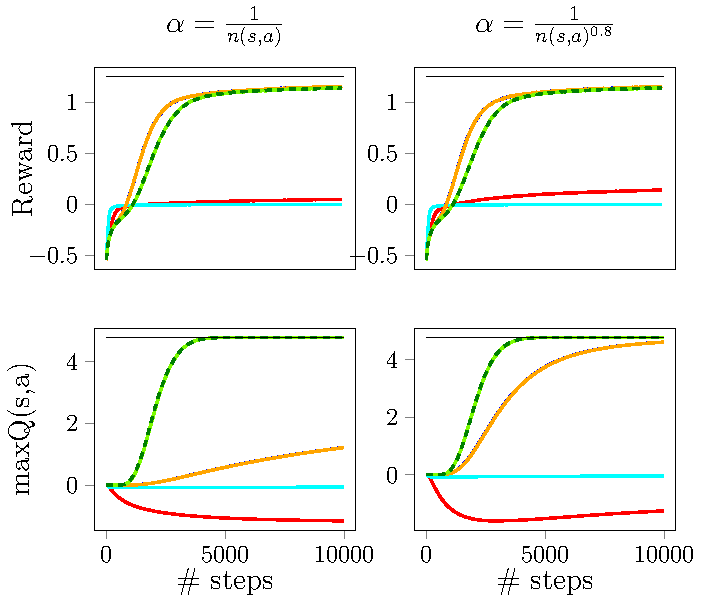
\includegraphics[scale=.7]{./img/grid_hole.pdf}
\end{minipage}
  \caption[Grid World with Holes algorithms comparison - 1]{Mean reward per step (top) and maximum action-value estimate in the Grid World with Holes problem in the initial state (bottom) of all the other algorithms and of the best setting of $RQ$-Learning for this experiment. Results are averaged over $10000$ experiments.}
  \label{F:hole}
\end{figure}

\begin{figure}[t]
\centering
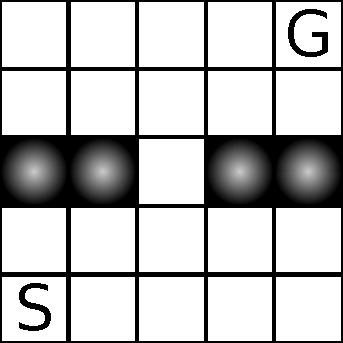
\includegraphics[scale=.55]{./img/gridhole.pdf}
\caption[Structure of the Grid World with Holes problem.]{Structure of the Grid World with Holes problem.}
  \label{F:grid_hole_map}
\end{figure}
This environment consists of a $5 \times 5$ grid with the initial position in the lower-left cell, there are $4$ actions and the transition model is deterministic, the goal position in the upper-right cell and four holes in the middle row in such a way that only the cell in the middle is walkable (Figure \ref{F:grid_hole_map}). The agent receives a reward of $0$ in all non-hole cells, a reward of $10$ when it reaches the goal state and a reward of $-10$ when it reaches a cell with a hole. The episode ends when the agent reaches a cell with a hole or the goal state. The discount factor is $\gamma = 0.9$. $RQ$-Learning uses $\eta = 1$.
The learning rate settings are the same as the previous problem.

We consider this simple problem to highlight the limitations of pessimistic action-value estimates. In this \gls{mdp}, the optimal policy consists in avoiding the hole cells stepping through the state in the middle. Notice that in this state the episode terminates with a negative reward with probability $\frac{\varepsilon}{2}$ due to the $\varepsilon$-greedy policy used for exploration, resulting in a very low value of the state, especially at the beginning of learning. Figure \ref{F:hole} shows that while $Q$-Learning, Speedy $Q$-Learning, and $RQ$-Learning behave similarly well, Double $Q$-Learning and Weighted $Q$-Learning obtain very poor results due to the pessimistic estimate of the value function of the state in the middle.
\begin{figure}[t]
\begin{minipage}{\columnwidth}
\centering
  \subfigure{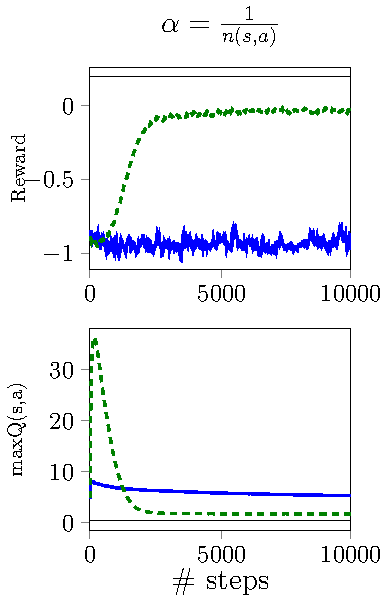
\includegraphics[scale=.7]{./img/sarsa1.pdf}}
  \subfigure{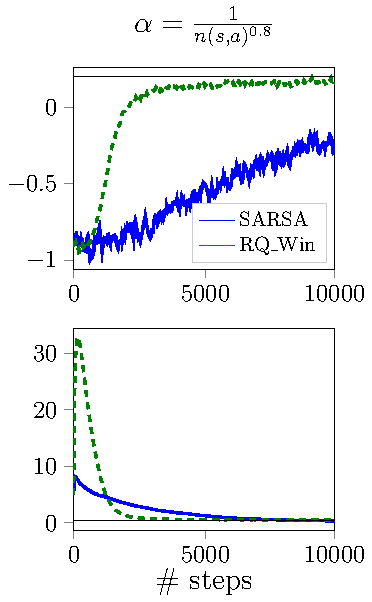
\includegraphics[scale=.7]{./img/sarsa08.pdf}}
\end{minipage}
  \caption[Grid World with Holes algorithms comparison - 2]{Mean reward per step (top) and maximum action-value estimate in the Noisy Grid World problem in the initial state (bottom) of SARSA and of the on-policy windowed version of $RQ$-Learning for this experiment. Results are averaged over $1000$ experiments.}
  \label{F:sarsa}
\end{figure}

\subsection{On-policy learning}
As we discussed in the previous sections, our approach can be used also in an on-policy setting. A simple on-policy version of our algorithm can be implemented by estimating the action-value function of the current policy in the same way of the SARSA algorithm, i.e. by using the action-value function of the next action. Let $a'$ be the next action sampled by the current policy in the current state, the on-policy update is:
\begin{align*}
\tilde{R}_{t+1}(s,a) & \leftarrow\tilde{R}_t(s,a)+\alpha_t(R(s,a,s')-\tilde{R}_t(s,a)),\\
\tilde{Q}_{t+1}(s,a) & \leftarrow\tilde{Q}_t(s,a)+\beta_t(Q_t(s',a')-\tilde{Q}_t(s,a)).
\end{align*}

Figure \ref{F:sarsa} compares the windowed, on-policy version of $RQ$-Learning with the SARSA algorithm, in the Noisy Grid World environment. It is clear that our algorithm outperforms SARSA in this \gls{mdp}.
Since this is an on-policy setting, at each step the algorithm is estimating the action-value function of the current policy, not the optimal one. Indeed, by looking at the average reward per step, our approach estimates the current action-value function of the policy better than the SARSA algorithm, i.e. the estimated action-value function is coherent with the performance of the policy.
